\documentclass[twocolumn]{article}
\usepackage[a4paper,margin=1in]{geometry}  % Adjust as needed
\usepackage{graphicx}
% \begin{figure*}
%     \centering
%     \includegraphics[width=\textwidth]{example-image}
%     \caption{A figure spanning both columns.}
%     \label{fig:example}
% \end{figure*}
\usepackage{lipsum}  % For placeholder text
\usepackage{microtype}  % Better text spacing
\usepackage{acronym}
\usepackage{hyperref}
\usepackage[utf8]{inputenc}
\usepackage{cleveref}
\usepackage[inline]{enumitem}

\acrodef{RL}{\textit{Reinforcement Learning}}
\acrodef{LLM}{Large Language Models}
\acrodef{CoALA}{\textbf{Co}gnitive \textbf{A}rchitectures for \textbf{L}anguage \textbf{A}gents}

\title{
\LARGE{\textbf{Analysis of \\ ''Cognitive Architecture for Language Agents``}}
\\[2ex] \textit{Software Architecture and Platforms} - A.Y. 2024/2025
}
\date{March 2025}
\author{Stefano Furi - \texttt{stefano.furi@studio.unibo.it} - 0001125057}

\begin{document}

\maketitle

\section{Introduction}\label{introduction}

\textbf{Language Agents} are an emerging class of AI systems that use \ac{LLM} to
interact with the world, applying advancements of current AI to the existing
field of agent design, offering benefits for both fields.
On one hand \ac{LLM}s have limited knowledge and reasoning capabilities,
mitigated by connecting an \ac{LLM}s to internal memory and environments. On the
other hand, traditional agents often require handcrafted rules or ,
making generalisation challenging.

Modern techniques of integrating \ac{LLM}s into the feedback loop of a
cognitive agent, use the \ac{LLM} to reason, plan and manage long-term memory
to improve \textbf{decision-making}. However, individual works use
custom terminology to describe these processes. This paper proposes a
conceptual framework in order to organise such efforts. The definition of such
framework is lead by two ideas coming from history of computing and AI:
\begin{itemize}
    \item \textbf{Production Systems} generate a set of outcomes by iteratively
    applying rules, originated as string manipulation systems;
    \item \textbf{Cognitive Agents}: in order for \emph{production systems} to
    be able to define systems capable of complex, hierarchically structured
    behaviours, they were \textbf{incorporated} into cognitive architectures,
    making it possibile to specify a \emph{control flow} for \emph{selecting},
    \emph{applying} and \emph{generating} new productions.
\end{itemize}

The paper then describes a possible driver in order to define control over \ac{LLM}
making them actual language agents, stating that as production systems indicate
possible ways for modifying strings and \ac{LLM}s define a distribution over changes
or additions to text, then \emph{control} from cognitive architectures used with
production systems might be equally applicable to transform \ac{LLM}s into
\emph{Language Agents}.

The authors then proposes \ac{CoALA}, a conceptual framework to characterise and
design general purpose language agents. Agents in CoALA are orgagnised along
three dimensions:
~\cite{sumers2024cognitivearchitectureslanguageagents}

\begin{itemize}
    \item \textbf{Information Storage}: \emph{working memory}, \emph{long-term memories};
    \item \textbf{Action Space}: \emph{internal} space, \emph{external space}
    \item \textbf{Decision-making Procedure}: interactive loop with \emph{planning} and \emph{execution}.
\end{itemize}

%!TEX root = ../main.tex
\section{Cognitive Architecture and LLMs Integration}\label{background}
\subsection{Production Systems}
In symbolic AI, when it comes to \emph{production
systems}~\cite{humanproblemsolving} we refer to the reduction of mathematics and
computation to \emph{symbolic manipulation} and more in general, production
systems have been proposed as a formalism to think about arbitrary logical
systems~\cite{Post1943-POSFRO} which later will be shown to be equivalent to a
simpler string rewriting system. Thanks to this approach, complex behaviours
could emerge from quite simple production systems. The large adoption by the AI
community of production systems came from their generalisation to
\textbf{logical operations}: \emph{preconditions} that could be checked against
agent's \emph{goals} and \emph{world} state, and \emph{actions} that should be
taken if preconditions are satisfied.

\subsection{Cognitive Architectures}
The usage of large production systems connected to external sensors, actuator
and knowledge bases, required a sophisticated control flow: a \textbf{Cognitive
Architecture}~\cite{LANGLEY2009141}. A typical Soar
Architecture~\cite{Newell1990-NEWUTO} as shown in \Cref{fig:soar}, is composed
by four major concepts:

\begin{figure*}[ht]
    \centering
    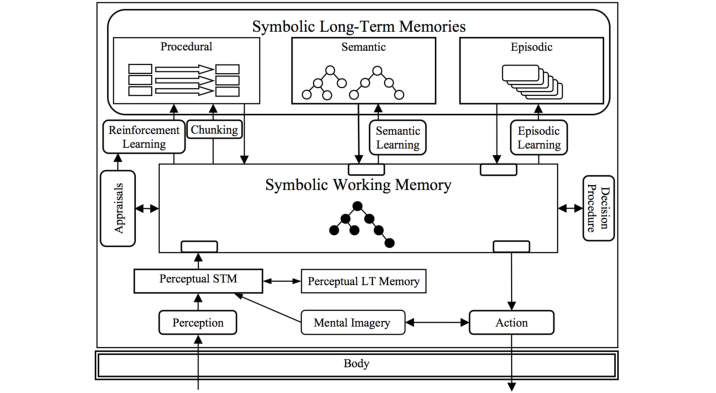
\includegraphics[width=\textwidth]{img/The-Soar-cognitive-architecture.png}
    \caption{The Soar Architecture}
    \label{fig:soar}
\end{figure*}

\begin{itemize}
    \item \textbf{Memory}: multiple memories, mainly divided into \emph{short
        term working memory} which reflects agent's current circumstances
        (perceptual inputs, goals, intermediate results), and a \emph{long term
        memory} which is divided into a
    \begin{enumerate*}[label=(\emph{\roman{*}})]
        \item \emph{procedural memory} containing the production system, a
        \item \emph{semantic memory} which stores facts about the world and the
            agent itself, and an
        \item \emph{episodic memory} keeping track of agent's past behaviours.
    \end{enumerate*}
    \item \textbf{Grounding}: in embodied context percepts are generated by
        sensors as agent's inputs, also equipping the Soar agent with actuators
        allowing physical interactions.
    \item \textbf{Decision Making} accomplished through a decision loop that
    \begin{enumerate*}[label=(\emph{\roman{*}})]
        \item matches preconditions from procedural memory,
        \item checks preconditions against agent's working memory,
        \item through a \emph{propose and evaluate phase} actions ranking and
            selections is performed for then
        \item choose, produce and execute the action.
    \end{enumerate*}
    \item \textbf{Learning} is supported by the Soar architecture through
        various forms, where in the most basic ways, facts are written in to
        semantic memory and experiences in episodic memory. Even behaviours can
        be modified by rewriting through \ac{RL} or adding new productions to
        the procedural memory.
\end{itemize}

Cognitive architectures have become less popular over the last few decades
reflecting two main problems: they're \emph{limited to domains} that can be
described with logical predicates, and require many pre-specified rules in order
to function properly.

\subsection{Language Models and Agents}
At its core, a language model is a probabilistic input-output system, where it
learn a distribution $P(w_i|w_{<i})$, where each $w$ is an individual
\emph{token} (word). With the rise of \textbf{Transformer
Based}~\cite{vaswani2023attentionneed} \ac{LLM}s with a large number of
parameters and smart tokenization schemes, along with training on
\emph{internet-scale} text, lead to models useful for many tasks beyond
generating text (e.g. writing code, , etc.). In scenarios where \ac{LLM}s act
in interactive environments, we talk about ''language agents``, i.e. systems
that uses \ac{LLM}s as a core computation unit to reason, plan and act.

\subsubsection{Connections between Language Models and Production Systems}
Formulating the problem of completing a piece of text as a production, allowing
multiple possible continuations, we have $X \rightarrow XY_i$ for some set of
$Y_i$. \ac{LLM}s assign a \emph{probability} to each of these completions.
From this perspective, they defines a probability distribution over \emph{which
productions} to select when presented with input $X$, yielding a distribution
$P(Y_i|X)$ over possible completion.

With this probabilistic approach:
\begin{itemize}
    \item \emph{disadvantages}: opaqueness, uninterpretable and random
        structure makes it challenging to analyze or control their behaviour;
    \item \emph{advantages}: scale and pre-training provide massive advantages
        over traditional production systems.
\end{itemize}

\subsubsection{From Prompt Engineering to Cognitive Language Agents}
Early work on few-shot learning and prompt engineering found that the \ac{LLM}
could be further biased towards high-quality productions by pre-processing the
input string. These manipulation can themselves be seen as productions.
Subsequent works used the \ac{LLM} itself as a pre-processing step, eliciting
targeted reasoning to foreground a particular aspect of the problem or generate
intermediate reasoning steps.

Moreover, when placing the \ac{LLM} in a \textbf{feedback loop} (e.g. Inner
Monologue~\cite{huang2022innermonologueembodiedreasoning} and
ReAct~\cite{yao2023reactsynergizingreasoningacting}) with the external
environment, generate systems that move beyond pre-defined prompt chains: they
first transform multimodal input into text and pass it to the \ac{LLM}, whose
output is then parsed and used to determine an external action.

Later work developed more sophisticated language agents that performs
intermediate reasoning by means of an \ac{LLM} before selecting an action, and
also incorporate learning strategies such as reflecting on episodic memory to
generate new semantic inferences, or modifying their procedural code to
generate new semantic knowledge.

Cognitive architecture has been used to structure production systems'
interactions with agents' internal state and external environment, and the
authors suggest that they can help design \ac{LLM}-based cognitive agents.

%!TEX root = ../main.tex
\section{The CoALA Framework}
\ac{CoALA} positions the \ac{LLM} as the core component of a larger cognitive
architecture, where a language agent stores information in \textbf{memory}
modules, and acts in an action space structured into external and internal
parts, as shown in \Cref{fig:coala}.
%
\begin{figure}[ht]
    \centering
    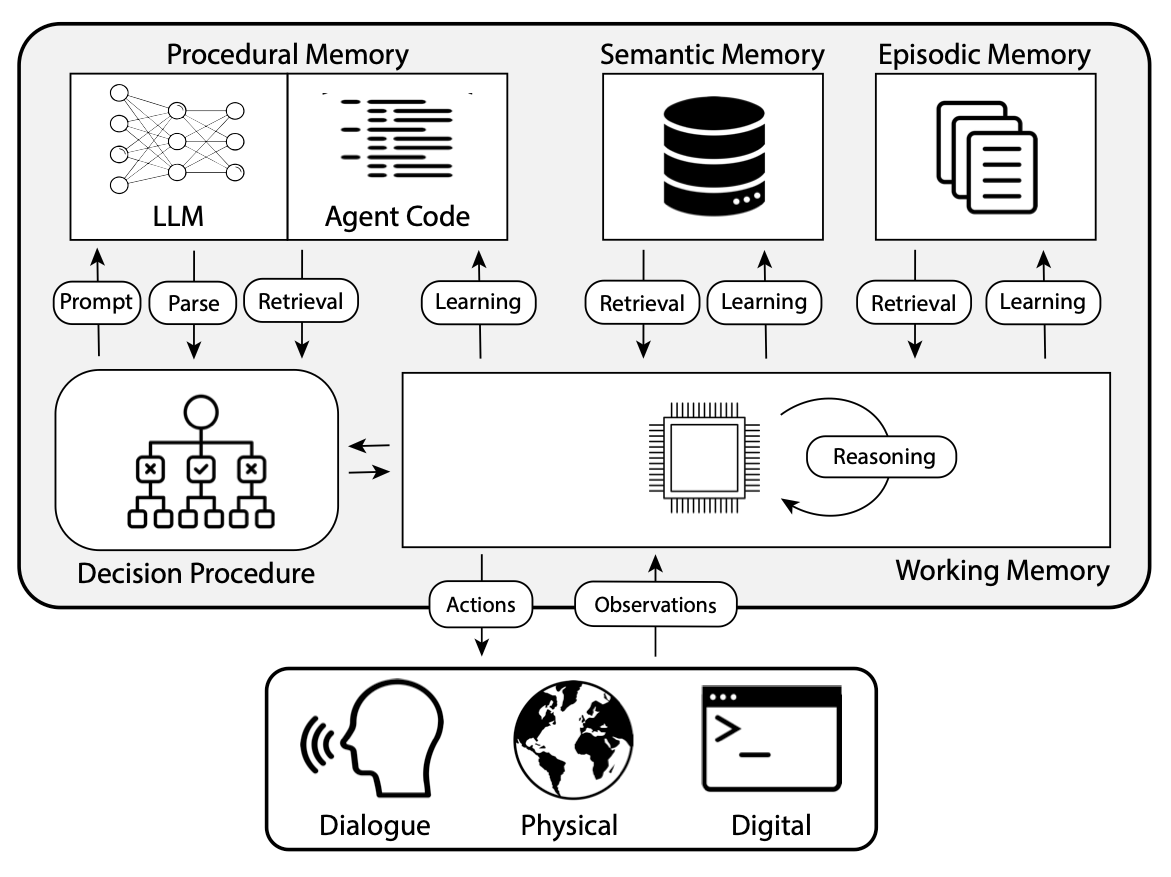
\includegraphics[width=0.4\textwidth]{img/coala-architecture.png}
    \caption{The \ac{CoALA} architecture, defining a set of interacting modules
    and processes.}
    \label{fig:coala}
\end{figure}
%
External actions let the agent interact with external environment through
\emph{grounding}, while internal actions consist of a set of interactions with
internal memories, and can be decomposed into
\begin{enumerate*}[label=(\emph{\roman{*}})]
    \item \emph{retrieval} when reading from long term memory,
    \item \emph{reasoning} with updates of the short term working memory with
        the \ac{LLM} and
    \item \emph{learning} by means of writing in long term memory.
\end{enumerate*}

\ac{CoALA} leverages key concepts inspired by decades of research in cognitive
agents, yet the incorporation of an \ac{LLM} lead to the addition of
\emph{reasoning actions}, which can \textbf{flexibly produce new knowledge} for
various purposes.

\subsection{Memory}
Memory is necessary due to the \emph{stateless} nature of \ac{LLM}s, which has
been already shown by language agents to improve drastically agent's and
accuracy. Under the \ac{CoALA} framework agents organise information into
multiple memory modules, which we'll describe in the following paragraphs.

\paragraph{Working Memory} maintains active and readily available information
for the \emph {current decision cycle}, including perceptual input, active
reasoning and other information carried by the previous decision cycle. In
short, the working memory synthesise \ac{LLM}s input from a subset of working
memory, and its output is then parsed back into other variables which are
stored back in working memory and used to execute the corresponding action.
Finally, the working memory also interact with long-term memories and
grounding.

\paragraph{Episodic Memory} stores experiences from earlier decision cycles
which can be encoded in various formats. This memory can then be accessed by
the working memory during the \emph{planning stage} of a decision cycle to
support \emph{reasoning}.

\paragraph{Semantic Memory} stores an agent's \emph{knowledge} about the
\emph{world} and \emph{itself}. In language agents this memory is not
fixed/read-only but agents can write new knowledge obtained from \ac{LLM}
reasoning as a form of learning (incrementally build up knowledge from
experience).

\paragraph{Procedural Memory} divided in two forms

\begin{itemize}
    \item \emph{implicit} knowledge stored in the \ac{LLM} weights;
    \item \textbf{explicit} knowledge written in the agent's code, furthermore
        divisible into \emph{procedures} which implement \emph{actions} (reasoning,
        retrieval grounding and learning), and \emph{procedures} that implement \emph{decision-making} itself.
\end{itemize}

Unlike other memories, procedural memory \textbf{must be initialised} by the
designer, and finally, even if possible, learning by writing new actions into
this memory is \emph{riskier} as it can easily introduce bugs or allow an
agents to subvert its designer's intentions.

\subsection{Grounding Actions}
Grounding procedures execute internal actions and \emph{process environmental
feedback} into working memory as text.

\paragraph{Physical Environment} it involves processing inputs into textual
observations, and affect the physical environments via robotic planners that
take \emph{language-based commands}. When it comes to perceptual inputs,
\textbf{vision-language models} are typically used to convert images into
text~\cite{alayrac2022flamingovisuallanguagemodel}, providing additional
context for the \ac{LLM}.

\paragraph{Dialogue with Humans or Other Agents} by means of classical
linguistic interaction can let the agent to accept new instructions or learn
from people, and for agents capable of generating language they can ask for
clarification, collaborate with multiple agents for social simulations or
collaborative task solving.

\paragraph{Digital Environment} including interactions with games, APIs, as well as
\emph{general code execution}, resulting in cheaper, faster and thus a more convenient
testbed for language agents.

\subsection{Retrieval Actions (Planning)}
Retrieval can be seen as a general procedure for reading information from long
term memories into working memory. We distinguish among various type of
retrieval:
\begin{itemize}
    \item \emph{Rule Based retrieval} useful for explicit memory organisation
        (e.g. designer's rules), providing deterministic result with limited
        flexibility and struggling with complex queries/fuzzy matches.
    \item \emph{Sparse Retrieval} relies on discrete representations, such as
        keywords or reverse indices. It is great for fast retrieval of factual
        information or structured knowledge, but struggles with \emph{semantic
        matching}.
    \item \emph{Dense Retrieval} is particularly useful for retrieving
        semantically relevant concepts. It uses continuous vector
        representations (\emph{embeddings}) and retrieves memories based on
        semantic similarities (e.g. nearest neighbours in a $d$-dimensional
        feature space), like
        BERT~\cite{devlin2019bertpretrainingdeepbidirectional} which uses a
        transformer-based embedding model.
\end{itemize}

\subsection{Reasoning Actions (Planning)}
Reasoning consists of a set of actions that aim to the processing of the
context of working memory to generate new information. With reasoning a
summarisation and distillation of core information inside working memory is
performed, gaining insights about most recent observations, most recent
trajectory and, optionally, information retrieved from long term memories.

Reasoning supports \emph{learning} by writing results in long term memory, and
\emph{decision making} by using the results as additional context for
subsequent \ac{LLM} calls.

\subsection{Learning}\label{ssec:learning}
Learning is essentially a writing process on long term memories, which includes
various kind of procedures explored in the following sections. This various
ways of learning allow language agents (e.g. with respect to \ac{RL} agents) to
learn rapidly by storing task-relevant language (quicker than parameter updates
for \ac{RL} agents).

\subsubsection{Updating Episodic Memory with Experience}
Following \ac{RL} common practice, store episodic trajectories to update a
\emph{parametric policy}. The experiences in this memory could be retrieved
later as examples and bases for reasoning and decision-making.

\subsubsection{Updating Semantic Memory with Knowledge}
Make use of \ac{LLM}s to reason about \emph{raw experiences} and store
resulting \emph{inference} in semantic memory (e.g. there's no dishwasher in
the room).

\subsubsection{Updating LLMs Parameters (Procedural Memory)}
Recall that \ac{LLM} weights represent a \textbf{implicit procedural
knowledge}. Weights can then be adjusted to an agent's domain by \emph{fine
tuning} during its lifetime, and this can be accomplished by supervised
learning, imitation learning, from environmental feedback or AI feedback,
typically using a measure of \emph{consistency} to select generations to fine
tune on~\cite{wang2023selfconsistencyimproveschainthought}. Fine tuning is a
costly form of Learning, but as training is becoming more efficient and some
optimised \ac{LLM}s techniques are being exploited, it may be possible to allow
language agent to autonomously determine when and how to fine-tune their
\ac{LLM}.

\subsubsection{Updating Agent's Code (Procedural Memory)}
\ac{CoALA} allows agents to update their source code; more in particular:
\begin{itemize}
    \item \textbf{Update reasoning} for example, infer prompt instructions
        (template) from input-output
        examples~\cite{zhou2023largelanguagemodelshumanlevel};
    \item \textbf{Update grounding actions}: notably current methods are limited
        to creating new code skills to interact with external environment.
    \item \textbf{Update retrieval}, not yet studied because it is considered a
        basic action designed with some fixed implementation; however \ac{LLM}s
        can perform distillation or use other techniques to learn \emph{better
        retrieval processes}.
    \item \textbf{Update learning} or \textbf{decision making} is theoretically
        possible, however risky for the agent's functionality and alignment.
\end{itemize}

\subsection{Decision Making}
\begin{figure}[ht]
    \centering
    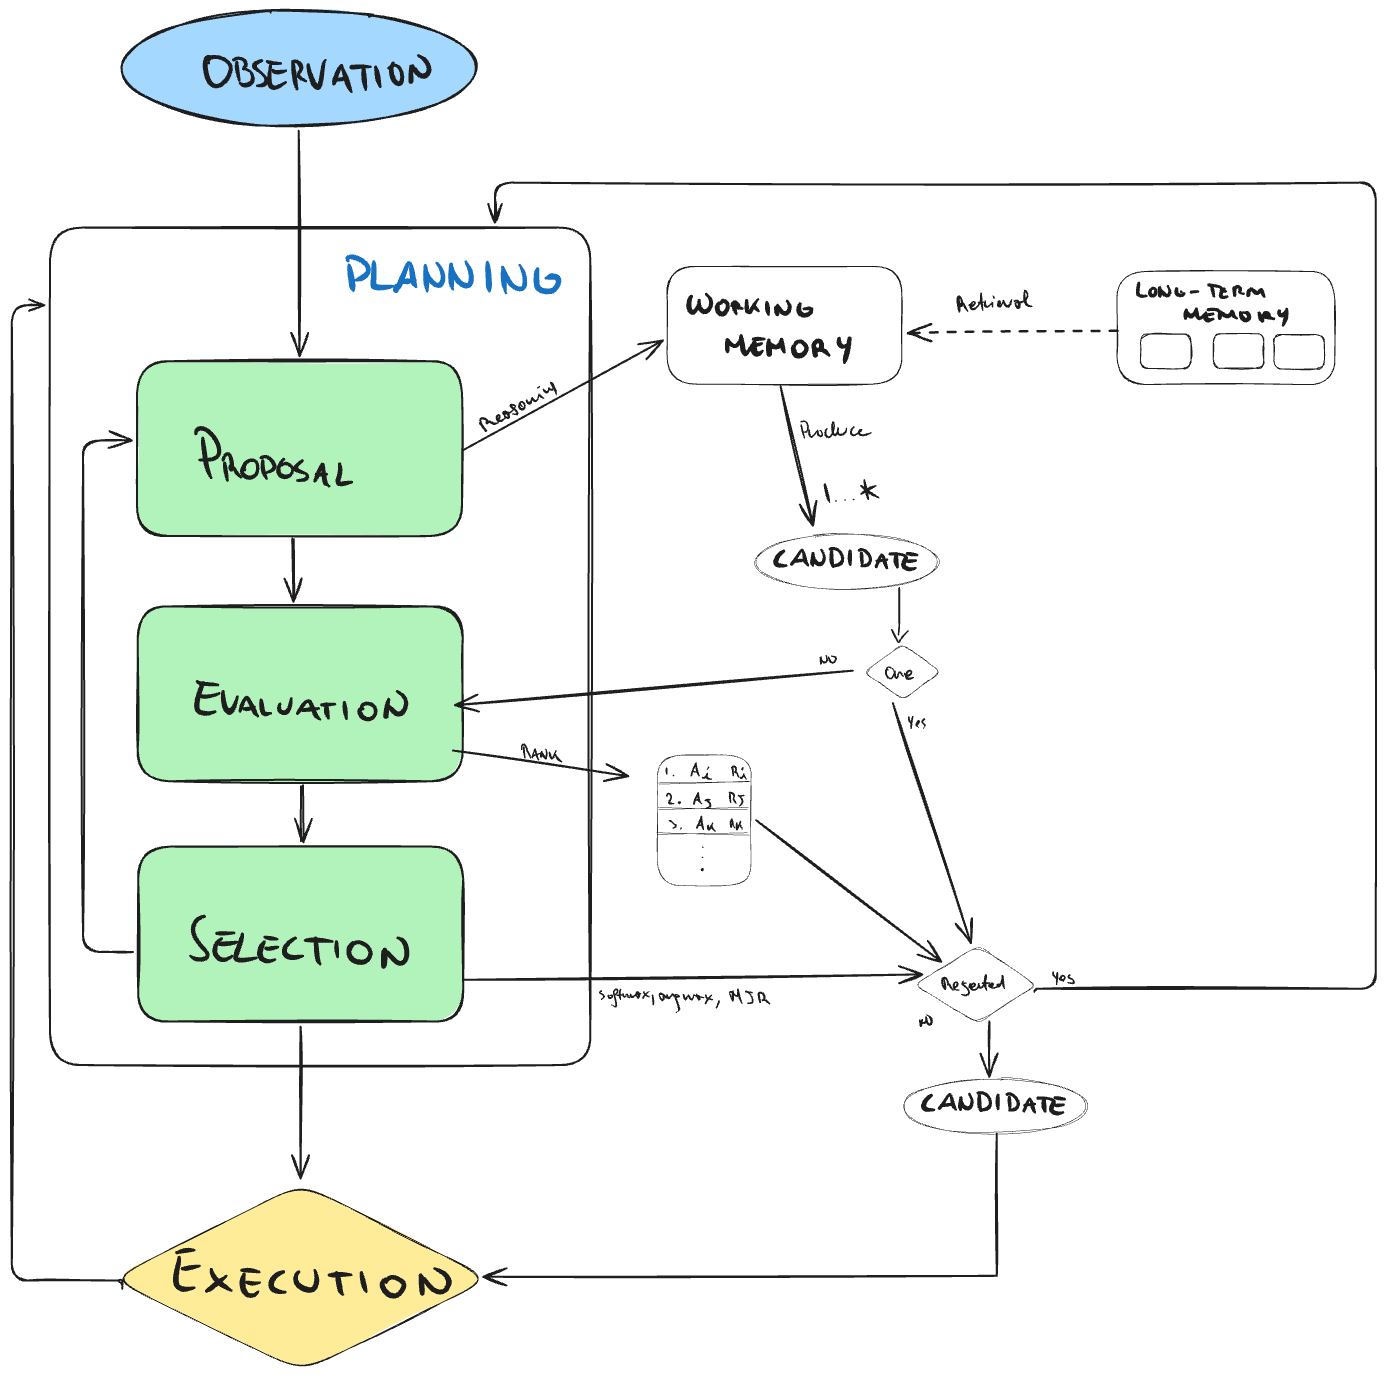
\includegraphics[width=0.4\textwidth]{img/coala-decision-making.pdf}
    \caption{The \ac{CoALA} decision making process, highlighting its building
        blocks (left) with the way they interact and interleave during the actual
        loop, by means of the decision tree (right).}
    \label{fig:coala-decision-making}
\end{figure}
Decision making is the procedure that chooses which action to apply, structured
into decision cycles which yield an external grounding action or internal
learning action.
In \Cref{fig:coala-decision-making} is shown the decision loop, integrated as well
with a simple custom decision tree. We can then summarise briefly its components:
\begin{itemize}
    \item \textbf{Planning Stage} where reasoning and retrieval can be applied
        to propose, evaluate and select actions. These sub-stages can iterate
        to build \emph{mulit-step} simulations before taking an action,
        improving at each cycle the candidate solution. Each cycle includes:
        \begin{enumerate}
            \item \emph{Proposal} where one or more action candidates are
                generated (using reasoning and optionally retrieval)a to sample
                one or more grounding actions from the \ac{LLM}.
            \item \emph{Evaluation} if multiple actions are proposed, for each
                one of them a value is assigned, either through heuristics,
                \ac{LLM} (perplexity) scores, or \ac{LLM} reasoning (useful for
                simulating grounding feedback from external
                world~\cite{hao2023reasoninglanguagemodelplanning})
            \item \emph{Selection} (through argmax, softmax or other like
                majority vote rule) of an action to execute, or reject them.
        \end{enumerate}
    \item \textbf{Execution}: selected action is applied executing relevant
        procedure from agent's source code. This can lead (depending on agent's
        implementation) to an external grounding action or an internal learning
        action.
\end{itemize}
%
After execution, an observation can be made from the environment, providing
feedback from the agent's action and the cycle loops again.

%!TEX root = ../main.tex
\section{Insights}
In the following section some actionable insights that have been considered as
particularly relevant are proposed and described.

\paragraph{Modular agents: thinking beyond monoliths.} Agents should be
\emph{structured and modular}, meaning that a framework for language agents
would consolidate technical investment and improve compatibility, both in
academic research by means of standardised terms and open source implementation
facilitating modular plug-and-play and re-use, and in industry application
maintaining a single company-wide ''language agent library`` reducing technical
dept facilitating testing and re-use, enabling end users to experience a context-specific
instanciation of the same base agent.

\paragraph{Agent design: thinking beyond simple reasoning.} \ac{CoALA} defines
agents over three different concepts (internal memory, set of possible internal
and external actions and a decision making procedure), thus when developing an
application-specific agent it consists of specifying implementations for each
of these components. More in particular:
\begin{itemize}
    \item \textbf{What memory modules are necessary}
    \item \textbf{Define agent's internal action space}, primarily consisting
        of defining read and write access to each of the agent's memory
        modules.
    \item\textbf{Define decision-making procedure} specifying how reasoning
        and retrieval actions are taken in order to choose an external or learning
        actions. This step requires a tradeoff between performance and
        generalisation.
\end{itemize}

\paragraph{Structured reasoning: thinking beyond prompt engineering.} \ac{CoALA} suggests
a more structured reasoning procedure to update working memory variables:
\begin{itemize}
    \item \textbf{Prompting frameworks} like
        LangChain\footnote{https://www.langchain.com} can be used to define
        higher-level sequences of reasoning steps, reducing the burden of
        reasoning per \ac{LLM} call and the low-level prompt crafting efforts.
    \item \textbf{Reasoning usecases in agents can inform and reshape LLM
        training} in terms of the types and formats of training instances.
        \ac{LLM}s trained or finetuned beyond NLP tasks and adapted towards
        different capabilities will more likely be the backbone of future
        agents.
\end{itemize}

\paragraph{Long-term memory: thinking beyond retrieval augmentation.}
Memory-augmented agents can both read and write self-generated content
autonomously, opening the way for efficient lifelong learning mechanisms such
as combining existing human knowledge with new experience and skills in order
to help agents bootstrap to learn efficiently, with, for example, auto
generation of episodic memory gaining knowledge from experience and reason
about it. More in general, the possibility of adaptive mechanisms interleaving
memory search and \emph{forward simulation} will allow agents to make the most
of their knowledge.

\paragraph{Learning: thinking beyond in-context learning or finetuning} by means of:
\begin{itemize}
    \item \textbf{Meta-learning by modifying agent's code}, for example
        learning better retrieval procedures or learning to reason about when
        certain knowledge would be useful.
    \item \textbf{New forms of learning (and unlearning)} could include
        fine-tuning \emph{smaller models} for specific reasoning sub-tasks and
        studying the interaction effects between multiple forms of learning.
\end{itemize}

\paragraph{Action space: thinking beyond external tools or actions.} A good
portion of agent's design should face the decision of the size and complexity
of the action space: larger and complex action space are very well performing
in complex scenarios, but they must face a more complex and sophisticated
decision-making problem, most of the time relying on more customised or
hand-crafted decision proceudres. A tradeoff of the action space vs.
decision-making complexities is a basic problem to be considered before
development, and as a general rule, taking the minimal action space necessary
to solve a given task might be preferred.
A non-negligible problem to address is the \emph{safety} of the actions space
for some actions that are inherently riskier. Today safety measures are
typically task specific heuristics.

\paragraph{Decision Making: thinking beyond action generation.} Current agents
have just scratched the surface of a more deliberate, propose-evaluate-select
decision making procedures.

\begin{itemize}
    \item \textbf{Mixing language based reasoning and code-based planning} may
        offer the best of both worlds, where agents may write and execute
        simulation code on the fly to evaluate the consequences of plans and
        plan using \ac{LLM}s to translate from natural language to structured
        world models.

    \item \textbf{Metareasoning to improve efficiency} considering that
        \ac{LLM}s calls are both slow and computationally intensive, and that
        there must be considered a balance between cost (computational and not)
        and the utility of the resulting improved plan, future work should
        develop mechanism to estimate the utility of planning (as humans seems
        to do).
\end{itemize} 

\paragraph{Calibration and Alignment.} More complex decision making is
currently bottlenecked by issues such as \emph{over-confidence} and
miscalibration, misalignment with human values or bias, hallucinations in
self-evaluation and lack of \emph{human-in-the-loop} mechanisms to face
uncertainties.



\bibliographystyle{alpha}
\bibliography{references}

\end{document}
